% % TikZ figure for SynthSAEBench overview
% % Requires: \usepackage{tikz}
% %           \usetikzlibrary{arrows.meta,positioning,fit,calc,shapes.geometric}

% \begin{tikzpicture}[
%     >=stealth,
%     treenode/.style={
%         circle,
%         draw,
%         minimum size=20pt,
%         inner sep=1pt,
%         font=\tiny
%     },
%     treeedge/.style={
%         draw,
%         thick
%     },
%     sectionlabel/.style={
%         font=\normalsize,
%         anchor=south
%     }
% ]

% % Section labels (above each panel)
% \node[sectionlabel] at (-4.5, 2.85) {Hierarchy};
% \node[sectionlabel] at (0, 2.85) {Correlation};
% \node[sectionlabel] at (4.5, 2.85) {Superposition};

% % ============ HIERARCHY SECTION ============
% % Tree nodes (centered horizontally at x = -4.5).
% % Node centers are inset by the 20pt node radius (~0.35 units) from the
% % Correlation/Superposition box edges (y in [-0.05, 2.7]) so the visible
% % circles align with the box top and bottom.
% \node[treenode] (animal) at (-4.5, 2.35) {Animal};
% \node[treenode] (dog)    at (-5.5, 1.35) {Dog};
% \node[treenode] (bird)   at (-3.5, 1.35) {Bird};
% \node[treenode] (poodle) at (-6.0, 0.35) {Poodle};
% \node[treenode] (husky)  at (-5.0, 0.35) {Husky};
% \node[treenode] (eagle)  at (-4.0, 0.35) {Eagle};
% \node[treenode] (hawk)   at (-3.0, 0.35) {Hawk};

% % Tree edges
% \draw[treeedge] (animal) -- (dog);
% \draw[treeedge] (animal) -- (bird);
% \draw[treeedge] (dog) -- (poodle);
% \draw[treeedge] (dog) -- (husky);
% \draw[treeedge] (bird) -- (eagle);
% \draw[treeedge] (bird) -- (hawk);

% % ============ CORRELATION SECTION ============
% % Correlation matrix - 5x5 grid (centered horizontally at x = 0)
% \def\cellsize{0.55}
% \def\matrixX{-1.375}
% \def\matrixY{-0.05}

% % Define colors
% \definecolor{darkblue}{RGB}{0,0,139}
% \definecolor{medblue}{RGB}{100,100,200}
% \definecolor{lightblue}{RGB}{200,200,255}
% \definecolor{vlightblue}{RGB}{230,230,255}
% \definecolor{vlightpink}{RGB}{255,245,245}
% \definecolor{lightpink}{RGB}{255,220,220}
% \definecolor{medpink}{RGB}{255,180,180}

% % Draw filled squares (row 0 = top row, row 4 = bottom row)
% % Row 0 (top)
% \fill[darkblue]   (\matrixX,             \matrixY+4*\cellsize) rectangle +(\cellsize, \cellsize);
% \fill[vlightblue] (\matrixX+\cellsize,   \matrixY+4*\cellsize) rectangle +(\cellsize, \cellsize);
% \fill[lightpink]  (\matrixX+2*\cellsize, \matrixY+4*\cellsize) rectangle +(\cellsize, \cellsize);
% \fill[vlightblue] (\matrixX+3*\cellsize, \matrixY+4*\cellsize) rectangle +(\cellsize, \cellsize);
% \fill[medpink]    (\matrixX+4*\cellsize, \matrixY+4*\cellsize) rectangle +(\cellsize, \cellsize);

% % Row 1
% \fill[vlightblue] (\matrixX,             \matrixY+3*\cellsize) rectangle +(\cellsize, \cellsize);
% \fill[darkblue]   (\matrixX+\cellsize,   \matrixY+3*\cellsize) rectangle +(\cellsize, \cellsize);
% \fill[vlightblue] (\matrixX+2*\cellsize, \matrixY+3*\cellsize) rectangle +(\cellsize, \cellsize);
% \fill[vlightpink] (\matrixX+3*\cellsize, \matrixY+3*\cellsize) rectangle +(\cellsize, \cellsize);
% \fill[vlightblue] (\matrixX+4*\cellsize, \matrixY+3*\cellsize) rectangle +(\cellsize, \cellsize);

% % Row 2
% \fill[lightpink]  (\matrixX,             \matrixY+2*\cellsize) rectangle +(\cellsize, \cellsize);
% \fill[vlightblue] (\matrixX+\cellsize,   \matrixY+2*\cellsize) rectangle +(\cellsize, \cellsize);
% \fill[darkblue]   (\matrixX+2*\cellsize, \matrixY+2*\cellsize) rectangle +(\cellsize, \cellsize);
% \fill[vlightblue] (\matrixX+3*\cellsize, \matrixY+2*\cellsize) rectangle +(\cellsize, \cellsize);
% \fill[lightpink]  (\matrixX+4*\cellsize, \matrixY+2*\cellsize) rectangle +(\cellsize, \cellsize);

% % Row 3
% \fill[vlightblue] (\matrixX,             \matrixY+\cellsize) rectangle +(\cellsize, \cellsize);
% \fill[vlightpink] (\matrixX+\cellsize,   \matrixY+\cellsize) rectangle +(\cellsize, \cellsize);
% \fill[vlightblue] (\matrixX+2*\cellsize, \matrixY+\cellsize) rectangle +(\cellsize, \cellsize);
% \fill[darkblue]   (\matrixX+3*\cellsize, \matrixY+\cellsize) rectangle +(\cellsize, \cellsize);
% \fill[vlightpink] (\matrixX+4*\cellsize, \matrixY+\cellsize) rectangle +(\cellsize, \cellsize);

% % Row 4 (bottom)
% \fill[medpink]    (\matrixX,             \matrixY) rectangle +(\cellsize, \cellsize);
% \fill[vlightblue] (\matrixX+\cellsize,   \matrixY) rectangle +(\cellsize, \cellsize);
% \fill[lightpink]  (\matrixX+2*\cellsize, \matrixY) rectangle +(\cellsize, \cellsize);
% \fill[vlightpink] (\matrixX+3*\cellsize, \matrixY) rectangle +(\cellsize, \cellsize);
% \fill[darkblue]   (\matrixX+4*\cellsize, \matrixY) rectangle +(\cellsize, \cellsize);

% % Draw outer border
% \draw[thin] (\matrixX, \matrixY) rectangle (\matrixX+5*\cellsize, \matrixY+5*\cellsize);

% % ============ SUPERPOSITION SECTION ============
% % Superposition box (centered horizontally at x = 4.5)
% \def\superSize{2.75}
% \def\superX{3.125}
% \def\superY{-0.05}

% % Draw box
% \draw[thin] (\superX, \superY) rectangle (\superX+\superSize, \superY+\superSize);

% % Draw dashed axes
% \draw[dashed, gray!60] (\superX+\superSize/2, \superY) -- (\superX+\superSize/2, \superY+\superSize);
% \draw[dashed, gray!60] (\superX, \superY+\superSize/2) -- (\superX+\superSize, \superY+\superSize/2);

% % Center point
% \pgfmathsetmacro{\cx}{\superX+\superSize/2}
% \pgfmathsetmacro{\cy}{\superY+\superSize/2}
% \def\radius{1.1}

% % Draw 6 vectors radiating from center, equally spaced (60 degrees apart)
% \definecolor{vecblue}{RGB}{30,100,200}

% \foreach \angle in {15, 75, 135, 195, 255, 315} {
%     \draw[vecblue, thick] (\cx, \cy) -- ({\cx+\radius*cos(\angle)}, {\cy+\radius*sin(\angle)});
%     \fill[vecblue] ({\cx+\radius*cos(\angle)}, {\cy+\radius*sin(\angle)}) circle (3pt);
% }

% \end{tikzpicture}

% TikZ figure for SynthSAEBench overview
% Requires: \usepackage{tikz}
%           \usetikzlibrary{arrows.meta,positioning,fit,calc,shapes.geometric}

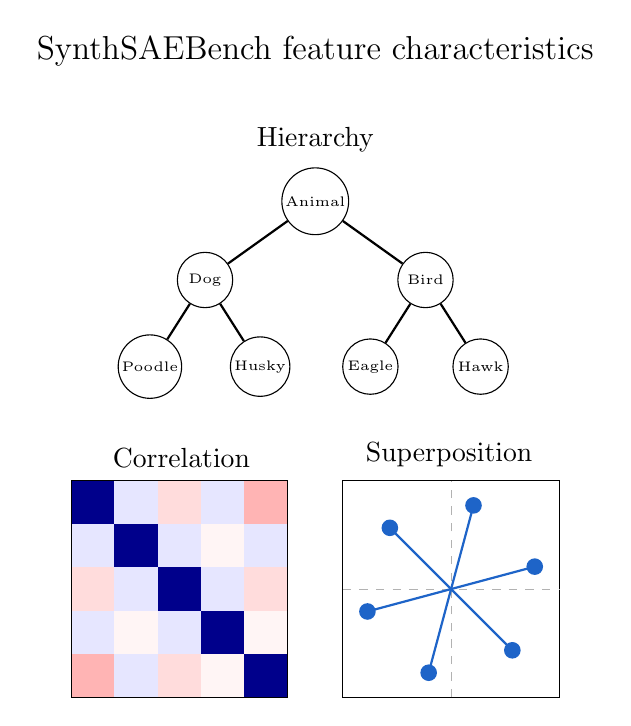
\begin{tikzpicture}[
    >=stealth,
    treenode/.style={
        circle,
        draw,
        minimum size=20pt,
        inner sep=1pt,
        font=\tiny
    },
    treeedge/.style={
        draw,
        thick
    },
    sectionlabel/.style={
        font=\normalsize,
        anchor=south
    }
]

% Title
\node[font=\large] at (0, 4.5) {SynthSAEBench feature characteristics};

% ============ HIERARCHY SECTION ============
\node[sectionlabel] at (0, 3.1) {Hierarchy};

% Tree nodes
\node[treenode] (animal) at (0, 2.6) {Animal};
\node[treenode] (dog) at (-1.4, 1.6) {Dog};
\node[treenode] (bird) at (1.4, 1.6) {Bird};
\node[treenode] (poodle) at (-2.1, 0.5) {Poodle};
\node[treenode] (husky) at (-0.7, 0.5) {Husky};
\node[treenode] (eagle) at (0.7, 0.5) {Eagle};
\node[treenode] (hawk) at (2.1, 0.5) {Hawk};

% Tree edges
\draw[treeedge] (animal) -- (dog);
\draw[treeedge] (animal) -- (bird);
\draw[treeedge] (dog) -- (poodle);
\draw[treeedge] (dog) -- (husky);
\draw[treeedge] (bird) -- (eagle);
\draw[treeedge] (bird) -- (hawk);

% ============ CORRELATION SECTION ============
% Label closer to the matrix
\node[sectionlabel] at (-1.7, -0.9) {Correlation};

% Correlation matrix - 5x5 grid
\def\cellsize{0.55}
\def\matrixX{-3.1}
\def\matrixY{-3.7}

% Define colors
\definecolor{darkblue}{RGB}{0,0,139}
\definecolor{medblue}{RGB}{100,100,200}
\definecolor{lightblue}{RGB}{200,200,255}
\definecolor{vlightblue}{RGB}{230,230,255}
\definecolor{vlightpink}{RGB}{255,245,245}
\definecolor{lightpink}{RGB}{255,220,220}
\definecolor{medpink}{RGB}{255,180,180}

% Draw filled squares (row 0 = top row, row 4 = bottom row)
% Row 0 (top)
\fill[darkblue] (\matrixX, \matrixY+4*\cellsize) rectangle +(\cellsize, \cellsize);
\fill[vlightblue] (\matrixX+\cellsize, \matrixY+4*\cellsize) rectangle +(\cellsize, \cellsize);
\fill[lightpink] (\matrixX+2*\cellsize, \matrixY+4*\cellsize) rectangle +(\cellsize, \cellsize);
\fill[vlightblue] (\matrixX+3*\cellsize, \matrixY+4*\cellsize) rectangle +(\cellsize, \cellsize);
\fill[medpink] (\matrixX+4*\cellsize, \matrixY+4*\cellsize) rectangle +(\cellsize, \cellsize);

% Row 1
\fill[vlightblue] (\matrixX, \matrixY+3*\cellsize) rectangle +(\cellsize, \cellsize);
\fill[darkblue] (\matrixX+\cellsize, \matrixY+3*\cellsize) rectangle +(\cellsize, \cellsize);
\fill[vlightblue] (\matrixX+2*\cellsize, \matrixY+3*\cellsize) rectangle +(\cellsize, \cellsize);
\fill[vlightpink] (\matrixX+3*\cellsize, \matrixY+3*\cellsize) rectangle +(\cellsize, \cellsize);
\fill[vlightblue] (\matrixX+4*\cellsize, \matrixY+3*\cellsize) rectangle +(\cellsize, \cellsize);

% Row 2
\fill[lightpink] (\matrixX, \matrixY+2*\cellsize) rectangle +(\cellsize, \cellsize);
\fill[vlightblue] (\matrixX+\cellsize, \matrixY+2*\cellsize) rectangle +(\cellsize, \cellsize);
\fill[darkblue] (\matrixX+2*\cellsize, \matrixY+2*\cellsize) rectangle +(\cellsize, \cellsize);
\fill[vlightblue] (\matrixX+3*\cellsize, \matrixY+2*\cellsize) rectangle +(\cellsize, \cellsize);
\fill[lightpink] (\matrixX+4*\cellsize, \matrixY+2*\cellsize) rectangle +(\cellsize, \cellsize);

% Row 3
\fill[vlightblue] (\matrixX, \matrixY+\cellsize) rectangle +(\cellsize, \cellsize);
\fill[vlightpink] (\matrixX+\cellsize, \matrixY+\cellsize) rectangle +(\cellsize, \cellsize);
\fill[vlightblue] (\matrixX+2*\cellsize, \matrixY+\cellsize) rectangle +(\cellsize, \cellsize);
\fill[darkblue] (\matrixX+3*\cellsize, \matrixY+\cellsize) rectangle +(\cellsize, \cellsize);
\fill[vlightpink] (\matrixX+4*\cellsize, \matrixY+\cellsize) rectangle +(\cellsize, \cellsize);

% Row 4 (bottom)
\fill[medpink] (\matrixX, \matrixY) rectangle +(\cellsize, \cellsize);
\fill[vlightblue] (\matrixX+\cellsize, \matrixY) rectangle +(\cellsize, \cellsize);
\fill[lightpink] (\matrixX+2*\cellsize, \matrixY) rectangle +(\cellsize, \cellsize);
\fill[vlightpink] (\matrixX+3*\cellsize, \matrixY) rectangle +(\cellsize, \cellsize);
\fill[darkblue] (\matrixX+4*\cellsize, \matrixY) rectangle +(\cellsize, \cellsize);

% Draw outer border
\draw[thin] (\matrixX, \matrixY) rectangle (\matrixX+5*\cellsize, \matrixY+5*\cellsize);

% ============ SUPERPOSITION SECTION ============
% Label closer to the box
\node[sectionlabel] at (1.7, -0.9) {Superposition};

% Superposition box
\def\superX{0.35}
\def\superY{-3.7}
\def\superSize{2.75}

% Draw box
\draw[thin] (\superX, \superY) rectangle (\superX+\superSize, \superY+\superSize);

% Draw dashed axes
\draw[dashed, gray!60] (\superX+\superSize/2, \superY) -- (\superX+\superSize/2, \superY+\superSize);
\draw[dashed, gray!60] (\superX, \superY+\superSize/2) -- (\superX+\superSize, \superY+\superSize/2);

% Center point
\pgfmathsetmacro{\cx}{\superX+\superSize/2}
\pgfmathsetmacro{\cy}{\superY+\superSize/2}
\def\radius{1.1}

% Draw 6 vectors radiating from center, equally spaced (60 degrees apart)
\definecolor{vecblue}{RGB}{30,100,200}

\foreach \angle in {15, 75, 135, 195, 255, 315} {
    \draw[vecblue, thick] (\cx, \cy) -- ({\cx+\radius*cos(\angle)}, {\cy+\radius*sin(\angle)});
    \fill[vecblue] ({\cx+\radius*cos(\angle)}, {\cy+\radius*sin(\angle)}) circle (3pt);
}

\end{tikzpicture}

